% 第 5 章 模型应用场景
\chapter{模型应用场景}

\begin{quote}
\textbf{本章范围声明}：本章描述推理服务在边缘侧容器化部署与运行的能力边界。推理框架由用户镜像自带，产品不内置；GPU/异构加速未验证。典型场景仅作通用示意，不承诺推理效果。
\end{quote}

\section{业务痛点}

\begin{itemize}
  \item \textbf{推理上云带宽压力大}：海量设备遥测、图像、信号数据持续上行至云端推理，带宽与流量成本随规模线性增长。
  \item \textbf{实时性不足}：数据往返云端再返回决策，时延无法满足实时监测、实时控制类业务的要求。
  \item \textbf{数据合规风险}：原始数据（图像、信号、工况）出域面临数据安全与合规压力，部分行业数据不允许离开本地网络。
  \item \textbf{边缘推理运维难}：推理实例多、分布广、环境异构，部署、升级、故障恢复依赖人工，运维负担重、可用性难保障。
\end{itemize}

\section{方案设计}

\textbf{总体思路}：将推理服务以容器化形式部署于边缘节点，与数据源同侧运行（\textbf{近数据侧推理}），构建“数据供给 $\rightarrow$ 推理消费 $\rightarrow$ 结果闭环”的本地推理链路；模型由第 4 章模型管理流程（镜像 + 配置）分发。

\textbf{组件与数据流}：

\begin{enumerate}
  \item \textbf{数据供给}：设备遥测经 MQTT 主题 \texttt{devices/<ns>/<device>/telemetry}（QoS1）供推理服务本地订阅（F28）；设备属性经属性 API 读取（F30）。
  \item \textbf{推理执行}：推理容器消费数据执行推理。\textbf{多副本}保证可用性（F12）、\textbf{健康自愈}保证持续服务（F13）、CrashLoopBackOff 退避避免重启风暴（F14）、\textbf{镜像漂移检测}防篡改（F15）、\textbf{断网自治}保证弱网/断网下推理容器持续运行（F16）。
  \item \textbf{结果闭环}：推理结果通过\textbf{设备命令闭环}触发设备动作（F23），或通过属性上报回写，形成“感知—推理—动作”闭环。
\end{enumerate}

\textbf{能力边界（如实标注）}：

\begin{itemize}
  \item 推理框架（TensorRT、ONNX Runtime 等）由用户镜像自带，\textbf{产品不内置}；
  \item \textbf{GPU/异构加速未验证}，当前以通用 CPU 算力承载推理负载。
\end{itemize}

\textbf{典型场景示意（通用示意，不承诺效果）}：设备预测性维护（基于工况遥测的异常检测与告警）、质量检测（图像/信号分类）。

\section{产品特性引用}

\textbf{表 5-1：模型应用场景特性引用}

{\small\setlength{\tabcolsep}{3pt}
\begin{tabular}{@{}p{1.6cm}p{0.8cm}p{3.4cm}p{8.8cm}@{}}
\toprule
环节 & F 编号 & 产品能力 & 说明\\
\midrule
容器生命周期管理 & F11 & 声明式调谐（5s 周期） & 推理实例按声明持续收敛，声明即运行态\\
 & F12 & 多副本补齐/收缩 & 推理服务多副本部署，单点故障自动补齐，可用性保障\\
 & F13 & 健康自愈自动重启 & 推理实例异常自动重启，保证持续服务\\
 & F14 & CrashLoopBackOff（3 次/30s 退避/60s 稳定重置） & 坏配置/坏镜像导致的连续失败进入退避，避免重启风暴\\
 & F15 & 镜像漂移检测自动重建 & 推理镜像被篡改/漂移时自动重建，防篡改\\
 & F16 & 断网自治容器持续运行 & 弱网/断网时推理容器持续运行，服务不中断\\
数据供给 & F28 & MQTT 遥测主题（QoS1） & 设备遥测数据本地订阅消费，作为推理输入\\
 & F30 & 设备属性 API & 读取设备属性，补充推理输入\\
结果闭环 & F21 / F22 & 影子与属性上报 & 推理结果/状态经影子汇聚与周期上报回写云端\\
 & F23 & 设备命令闭环 & 推理结果触发设备命令/动作，形成闭环\\
期望态持久化 & F17 & 边缘 MetaManager SQLite 持久化 & 数据订阅配置与期望态落盘，重启后不丢失\\
\bottomrule
\end{tabular}}

\section{部署方式}

\begin{figure}[htbp]
  \centering
  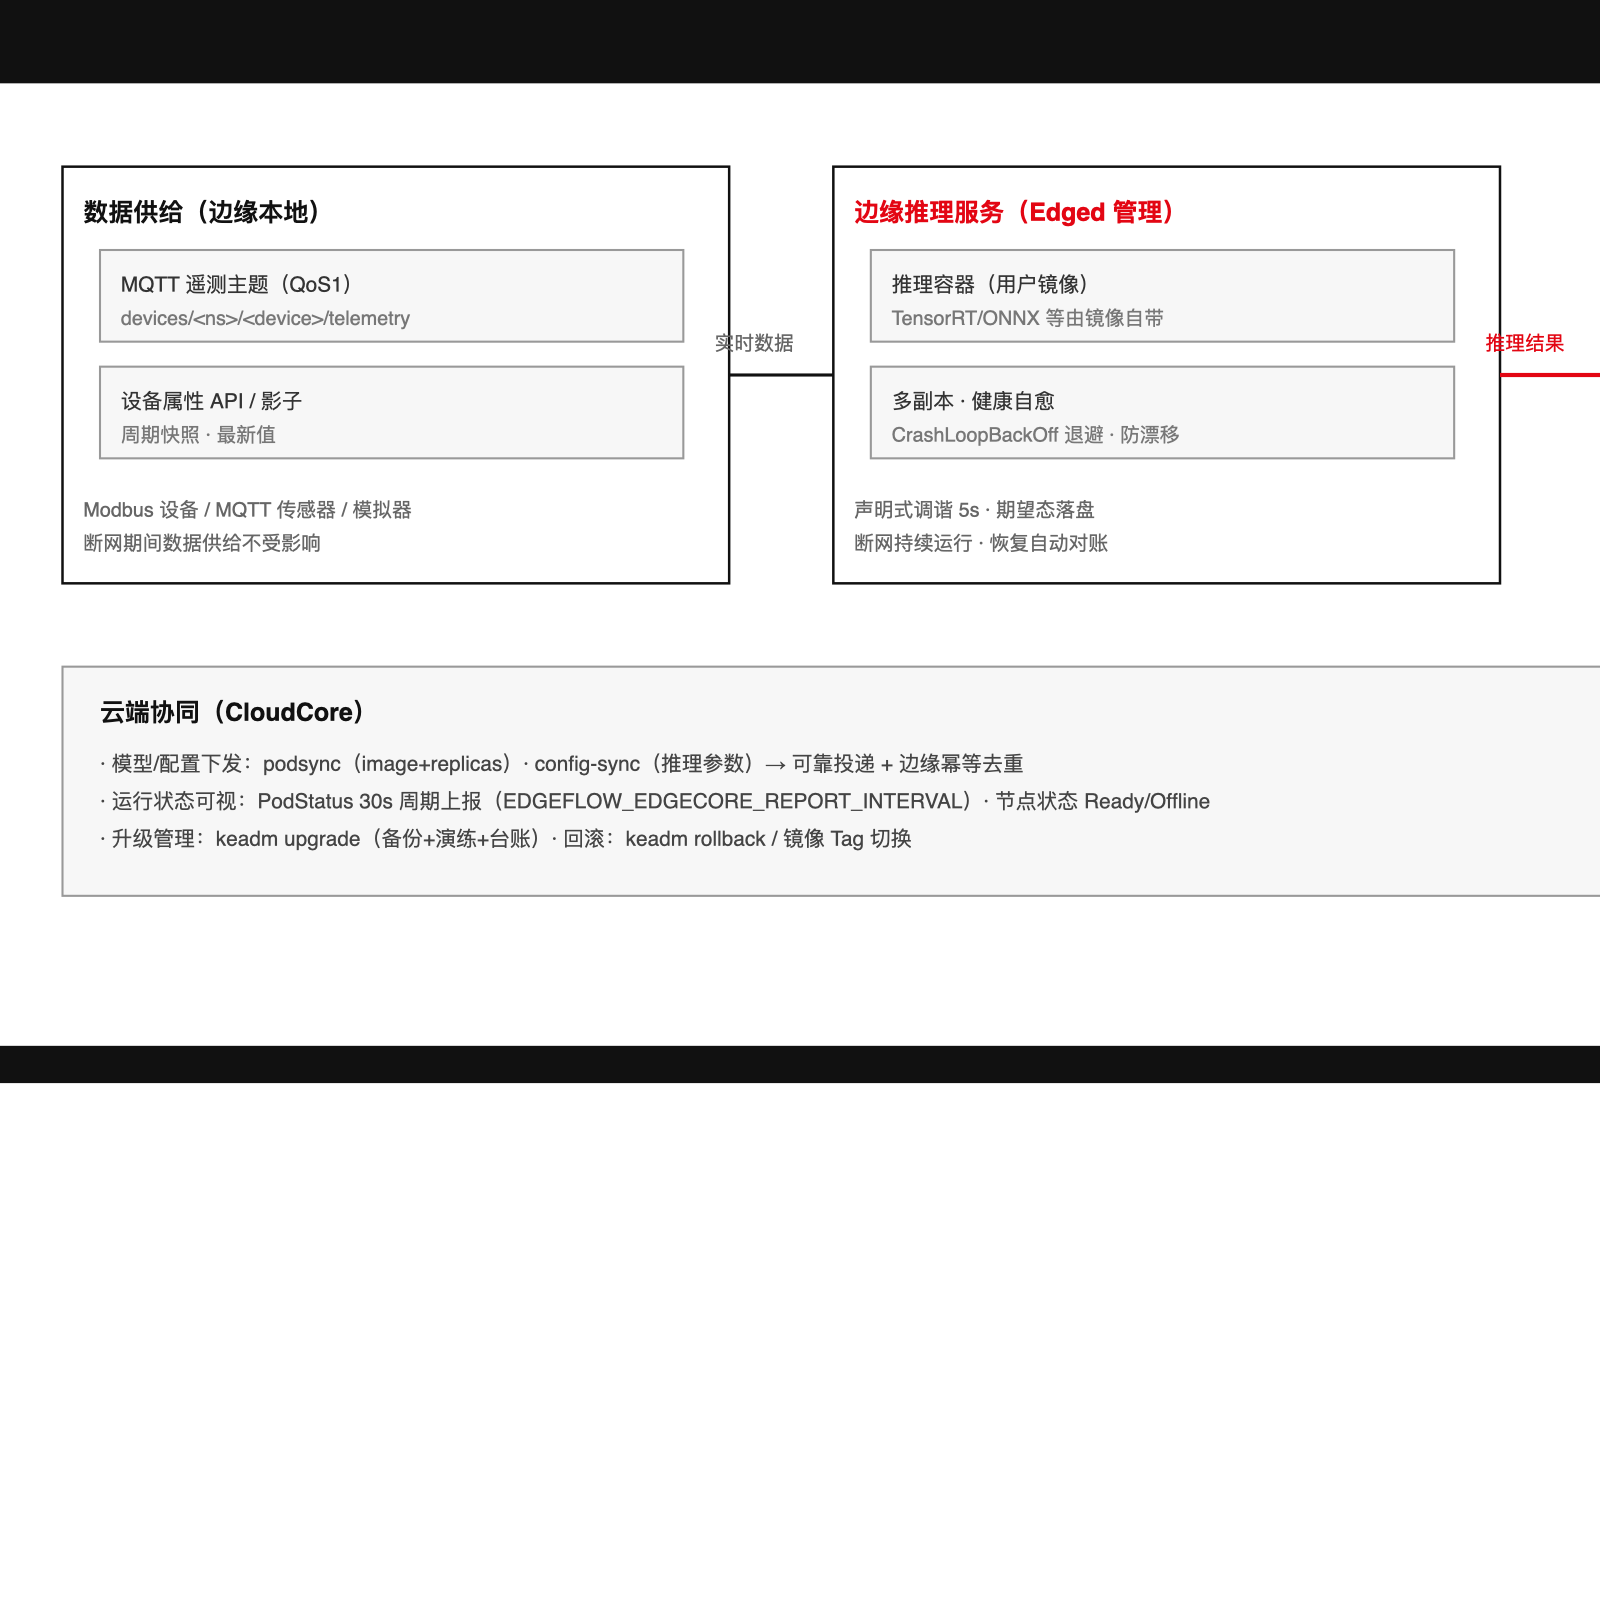
\includegraphics[width=0.94\textwidth]{../diagrams/scenario-model-app.png}
  \caption{模型应用场景：边缘推理部署拓扑}
  \label{fig:model-app}
\end{figure}

\textbf{（1）推理服务声明}（YAML 风格，字段示意；完整声明格式以产品文档为准）：

\begin{lstlisting}
# 推理服务声明（示意）
image:   registry.example.com/edgeflow/models/defect-detector:v1.2.0
replicas: 2
# 由 POST /api/v1/nodes/{nodeID}/podsync 下发（F31）
\end{lstlisting}

\textbf{（2）推理参数配置}：经 config-sync 下发（如告警阈值、推理超参），边缘 SQLite 持久化（F17）。

\textbf{（3）数据订阅配置}：推理容器订阅 \texttt{devices/<ns>/<device>/telemetry}（QoS1，F28）消费实时遥测；需要历史/聚合输入时经属性 API 读取（F30）。

\textbf{（4）多副本与自愈验证}：

\begin{itemize}
  \item 声明 replicas=2 后，Edged 在 5s 调谐周期内补齐副本（F11/F12）；
  \item 手动终止一个推理容器，观察自动重启（F13）与 RestartCount 累计；连续崩溃进入 CrashLoopBackOff 退避（F14）；
  \item 篡改推理镜像后观察漂移检测自动重建（F15）；
  \item 停 cloudcore 60s，观察推理容器持续运行（F16，E2E 短时验证口径同第 3 章）。
\end{itemize}

\textbf{（5）结果闭环验证}：推理结果触发 \texttt{POST /api/v1/nodes/\{nodeID\}/device-command} 下发设备动作（F23），或经属性上报在 \texttt{GET /api/v1/devices} 可见（F30）。

\section{客户价值}

\begin{itemize}
  \item \textbf{低时延本地推理}：推理与数据源同侧，数据不出本地网络即可完成决策，规避上云往返时延。
  \item \textbf{持续可用}：多副本 + 健康自愈 + 断网自治，推理服务在弱网/断网与实例故障下持续提供服务。
  \item \textbf{自动运维}：声明式调谐、自愈、退避与防漂移机制减少人工运维，边缘推理规模化可控。
  \item \textbf{数据不出域}：原始数据本地消费，满足数据安全与合规要求（结果性描述）。
\end{itemize}
